\task{Transient Performance Comparison of P1 Hybrid Sportscar with Task 2 and Task 3 Engines}
\label{ch:task4}

\section{Introduction}

Task~4 represents the final stage of the integrated powertrain development workflow, extending the steady-state engine performance from Tasks~1--3 to a fully transient, vehicle-level analysis within the AVL~CRUISE~M environment~\cite{avl_cruise}. This stage translates the AVL~BOOST steady-state results~\cite{avl_boost} into a dynamic context where control strategies and real-time subsystem interactions are evaluated under realistic driving conditions.

\vspace{0.8em}

The principal objective is to develop, calibrate, and validate a complete powertrain control strategy for a P1 hybrid electric vehicle model, including gear-shift logic optimization, hybrid control unit (HCU) coordination, and fuel-consumption map integration. The CRUISE~M model enables simulation of transient system behavior during rapid acceleration events.

\vspace{0.8em}

The primary comparison evaluates how the fundamentally different torque characteristics of the Task~2 naturally aspirated 2.0L engine (peak torque at 6500--8000~rpm) versus the Task~3 turbocharged 1.0L engine (peak torque at 3500~rpm) influence acceleration performance when integrated with the P1 electric motor system. These distinct characteristics necessitate different gear ratio strategies and shifting schedules to optimize 0--100~mph acceleration time.

\section{Model Overview}

\subsection{Vehicle Specifications}

The simulated vehicle is a two-seat front-wheel drive hybrid sportscar with specifications defined in Appendix~A of the assignment brief. The key vehicle parameters used in the AVL~CRUISE~M model are summarized in Table~\ref{tab:vehicle_specs}.

\begin{table}[H]
\centering
\caption{Vehicle Specifications for Task~4 Simulation}
\label{tab:vehicle_specs}
\small
\begin{tabular}{@{}lll@{}}
\toprule
\textbf{Parameter} & \textbf{Value} & \textbf{Unit} \\
\midrule
Total Vehicle Mass (full tank) & 720 & kg \\
Weight Distribution & 50\% Front / 50\% Rear & - \\
Wheelbase & 2300 & mm \\
Front Track & 1440 & mm \\
Rear Track & 1453 & mm \\
Tyre Size (Front \& Rear) & 195/65~R15 & - \\
Rolling Radius (Front) & 284 & mm \\
Rolling Radius (Rear) & 297 & mm \\
Height of Centre of Gravity & 470 & mm \\
Drag Coefficient & 0.418 & - \\
Frontal Area & 1.62 & m$^2$ \\
Final Drive Ratio & 3.938 & - \\
\bottomrule
\end{tabular}
\end{table}

The vehicle architecture follows a P1 hybrid configuration, where the electric motor is positioned between the internal combustion engine and the clutch, allowing both power sources to contribute to propulsion through the same driveline. The model assumes the vehicle is fully fuelled with no driver or passenger mass included beyond the base vehicle mass.

\subsection{Tyre Friction Limits}

The combined ICE and EM torque output must not exceed the traction limits of the front-wheel drive configuration. The maximum longitudinal tyre forces are determined using the load sensitivity relationship from Appendix~A. With 50:50 weight distribution and 720~kg total mass, the static front axle load is approximately 1.765~kN per wheel. During acceleration, load transfer reduces the grip of the front axle, which requires careful calibration of the EM output to avoid exceeding traction limits during high-torque launch phases.

\section{Task 2 Configuration: 2.0L Naturally Aspirated Engine with P1 Hybrid}

\subsection{Engine Specifications and Characteristics}

The Task~2 engine is a 2.0-litre, 4-cylinder inline naturally aspirated gasoline direct injection (GDi) engine optimized for high-RPM motorsport performance. As detailed in Task~2, this engine features a 1--3--4--2 firing order, semi-4-2-1 exhaust system, and variable cam phasing to achieve optimal breathing characteristics across the 2000--8000~rpm operating range.

\begin{table}[H]
\centering
\caption{Task~2 Engine Key Performance Parameters}
\label{tab:task2_engine_summary}
\small
\begin{tabular}{@{}lll@{}}
\toprule
\textbf{Parameter} & \textbf{Value} & \textbf{Unit} \\
\midrule
Displacement & 2.0 & litres \\
Configuration & Inline 4-cylinder & - \\
Aspiration & Naturally Aspirated & - \\
Peak Power & 175.5 & kW \\
Peak Power RPM & 8000 & rpm \\
Peak Torque & $\sim$220 & Nm \\
Peak Torque RPM & 6500--7000 & rpm \\
Operating Range & 2000--8000 & rpm \\
Fuel Type & Premium Unleaded (98 RON) & - \\
\bottomrule
\end{tabular}
\end{table}

The engine's high-RPM characteristic requires careful gear ratio selection to maintain the engine within its optimal operating window during transient acceleration. The naturally aspirated configuration delivers more linear torque with RPM compared to the turbocharged Task~3 variant, requiring electric motor low-end torque augmentation for improved launch performance.

\subsection{Electric Motor Specification and Integration}

The P1 electric motor selected for this application is the Valeo 48V water-cooled permanent magnet synchronous motor (PMSM)~\cite{valeo_48v_motor}, designed specifically for mild hybrid P1/P2 applications. The motor specifications are detailed in Table~\ref{tab:em_specs}.

\begin{table}[H]
\centering
\caption{Valeo 48V P1 Electric Motor Specifications~\cite{valeo_48v_motor}}
\label{tab:em_specs}
\small
\begin{tabular}{@{}lll@{}}
\toprule
\textbf{Parameter} & \textbf{Value} & \textbf{Unit} \\
\midrule
Peak Power & 25 & kW \\
Continuous Power & 15 & kW \\
Peak Torque & 170--180 & Nm \\
Voltage & 48 & V \\
Configuration & Water-cooled PMSM & - \\
Maximum Speed & 8000 & rpm \\
Application & P1/P2 Hybrid & - \\
\bottomrule
\end{tabular}
\end{table}

\subsection{EM Power Envelope Adaptation for Task 2}

The electric motor power envelope is calibrated to ensure the combined ICE and EM torque does not exceed front-wheel drive traction limits during launch and low-speed acceleration. The strategy considers three phases:

\begin{enumerate}
    \item \textbf{Traction-limited (0--40 mph):} Maximum EM boost (170--180~Nm) during launch, progressively reducing as load transfer diminishes front axle grip.
    \item \textbf{Power-limited (40--80 mph):} EM modulated to maintain total tractive force below friction limits.
    \item \textbf{High-speed (80--100 mph):} Both ICE and EM operate at peak capabilities as aerodynamic drag dominates.
\end{enumerate}

Simulations confirmed peak longitudinal forces remain within the friction envelope throughout acceleration, with maximum forces during 2nd and 3rd gear upshifts.

\subsection{Gear Ratio Optimization}

The gear ratios were optimized specifically for the Task~2 engine's high-RPM power delivery characteristic. The optimization objective was to maintain engine operation within the 6500--8000~rpm range during full-throttle acceleration, where both power and torque are maximized. The optimized transmission ratios are presented in Table~\ref{tab:task2_gear_ratios}.

\begin{table}[H]
\centering
\caption{Optimized Gear Ratios for Task~2 Configuration}
\label{tab:task2_gear_ratios}
\small
\begin{tabular}{@{}cccc@{}}
\toprule
\textbf{Gear} & \textbf{Baseline} & \textbf{Optimized} & \textbf{Overall Ratio} \\
\midrule
1 & 2.583 & \textcolor{optimizedcolor}{\textbf{3.4}} & 13.39 \\
2 & 2.071 & \textcolor{optimizedcolor}{\textbf{2.2}} & 8.66 \\
3 & 1.688 & \textcolor{optimizedcolor}{\textbf{1.6}} & 6.30 \\
4 & 1.412 & \textcolor{optimizedcolor}{\textbf{1.3}} & 5.12 \\
5 & 1.200 & \textcolor{optimizedcolor}{\textbf{1.0}} & 3.94 \\
6 & 1.048 & \textcolor{optimizedcolor}{\textbf{0.8}} & 3.15 \\
\bottomrule
\end{tabular}
\end{table}

The ratio progression reflects the following design considerations:

\begin{itemize}
    \item \textbf{First gear (3.4):} Strong launch torque multiplication while avoiding excessive wheel spin.
    \item \textbf{Second gear (2.2):} Large ratio drop (35\%) keeps engine above 5500~rpm after 1--2 upshift.
    \item \textbf{Third through fifth gears (1.6, 1.3, 1.0):} Tighter progression (18--23\% drops) maintains engine within 6500--8000~rpm power band.
    \item \textbf{Sixth gear (0.8):} Overdrive for cruise efficiency, not utilized during 0--100~mph acceleration.
\end{itemize}

\subsection{Shifting Strategy Development}

\subsubsection{Baseline Dummy Shifting Analysis}

The initial AVL~CRUISE~M model employed a "dummy" shifting strategy with fixed shift points that did not account for the engine's optimal power band. Analysis of the baseline performance revealed several inefficiencies through examination of the transient response characteristics.

\begin{figure}[H]
    \centering
    \begin{tikzpicture}
        \begin{axis}[
            width=0.75\textwidth,
            height=0.45\textwidth,
            xlabel={Time (s)},
            ylabel={Vehicle Speed (km/h) / Gear Level},
            ylabel style={font=\footnotesize},
            xlabel style={font=\footnotesize},
            tick label style={font=\footnotesize},
            grid=major,
            legend pos=north west,
            legend style={font=\tiny},
            xmin=0, xmax=16,
            ymin=0, ymax=200,
            axis y line*=left,
        ]
            \addplot[baselinecolor, thick, no markers] table[x index=0, y index=1, col sep=comma, skip first n=2] {task4/data/eng2/1_baseline_new_motor/velocity_rpm_gear.csv};
            \addlegendentry{Vehicle Speed}
            \addplot[improvementcolor, thick, const plot, no markers] table[x index=0, y expr=\thisrowno{2}*20, col sep=comma, skip first n=2] {task4/data/eng2/1_baseline_new_motor/velocity_rpm_gear.csv};
            \addlegendentry{Gear Level ($\times$20)}
        \end{axis}
        \begin{axis}[
            width=0.75\textwidth,
            height=0.45\textwidth,
            xlabel={Time (s)},
            ylabel={Engine Speed (rpm)},
            ylabel style={font=\footnotesize, red},
            xlabel style={font=\footnotesize},
            tick label style={font=\footnotesize},
            legend pos=south east,
            legend style={font=\tiny},
            xmin=0, xmax=16,
            ymin=0, ymax=8500,
            axis y line*=right,
            axis x line=none,
        ]
            \addplot[optimizedcolor, thick, no markers] table[x index=0, y index=3, col sep=comma, skip first n=2] {task4/data/eng2/1_baseline_new_motor/velocity_rpm_gear.csv};
            \addlegendentry{Engine Speed}
        \end{axis}
    \end{tikzpicture}
    \caption{Task~2 Baseline: Combined view of vehicle speed, engine speed, and gear progression with dummy shifting strategy}
    \label{fig:task2_baseline_combined}
\end{figure}

\subsubsection{Stage 1: Standard Shifting Strategy Implementation}

The first optimization stage implemented a basic RPM-based shifting strategy to improve upon the dummy baseline.

\begin{figure}[H]
    \centering
    \begin{tikzpicture}
        \begin{axis}[
            width=0.75\textwidth,
            height=0.45\textwidth,
            xlabel={Time (s)},
            ylabel={Vehicle Speed (km/h) / Gear Level},
            ylabel style={font=\footnotesize},
            xlabel style={font=\footnotesize},
            tick label style={font=\footnotesize},
            grid=major,
            legend pos=north west,
            legend style={font=\tiny},
            xmin=0, xmax=16,
            ymin=0, ymax=200,
            axis y line*=left,
        ]
            \addplot[baselinecolor, thick, no markers] table[x index=0, y index=1, col sep=comma, skip first n=2] {task4/data/eng2/2_standard_shifting/velocity_rpm_gear.csv};
            \addlegendentry{Vehicle Speed}
            \addplot[improvementcolor, thick, const plot, no markers] table[x index=0, y expr=\thisrowno{2}*20, col sep=comma, skip first n=2] {task4/data/eng2/2_standard_shifting/velocity_rpm_gear.csv};
            \addlegendentry{Gear Level ($\times$20)}
        \end{axis}
        \begin{axis}[
            width=0.75\textwidth,
            height=0.45\textwidth,
            xlabel={Time (s)},
            ylabel={Engine Speed (rpm)},
            ylabel style={font=\footnotesize, red},
            xlabel style={font=\footnotesize},
            tick label style={font=\footnotesize},
            legend pos=south east,
            legend style={font=\tiny},
            xmin=0, xmax=16,
            ymin=0, ymax=8500,
            axis y line*=right,
            axis x line=none,
        ]
            \addplot[optimizedcolor, thick, no markers] table[x index=0, y index=3, col sep=comma, skip first n=2] {task4/data/eng2/2_standard_shifting/velocity_rpm_gear.csv};
            \addlegendentry{Engine Speed}
        \end{axis}
    \end{tikzpicture}
    \caption{Task~2 Stage 1: Combined view of vehicle speed, engine speed, and gear progression}
    \label{fig:task2_stage1_combined}
\end{figure}

\begin{figure}[H]
    \centering
    \begin{tikzpicture}
        \begin{axis}[
            width=0.75\textwidth,
            height=0.45\textwidth,
            xlabel={Time (s)},
            ylabel={Vehicle Speed (km/h)},
            xlabel style={font=\footnotesize},
            ylabel style={font=\footnotesize},
            tick label style={font=\footnotesize},
            grid=major,
            legend pos=south east,
            legend style={font=\tiny},
            xmin=0, xmax=16,
            ymin=0, ymax=200,
        ]
            \addplot[baselinecolor, thick, no markers] table[x index=0, y index=1, col sep=comma, skip first n=2] {task4/data/eng2/1_baseline_new_motor/velocity_rpm_gear.csv};
            \addlegendentry{Baseline}
            \addplot[optimizedcolor, thick, no markers] table[x index=0, y index=1, col sep=comma, skip first n=2] {task4/data/eng2/2_standard_shifting/velocity_rpm_gear.csv};
            \addlegendentry{Standard Shifting}
        \end{axis}
    \end{tikzpicture}
    \caption{Task~2 Stage 1: Velocity comparison - Baseline vs Standard Shifting}
    \label{fig:task2_stage1_comparison}
\end{figure}

\begin{table}[H]
\centering
\caption{Task~2 Stage 1 Performance Summary: Baseline vs Standard Shifting}
\label{tab:task2_stage1_performance}
\small
\begin{tabular}{@{}lcccc@{}}
\toprule
\textbf{Metric} & \textbf{Baseline} & \textbf{Standard Shifting} & \textbf{Change} & \textbf{\% Change} \\
\midrule
0--100 kph time (s) & N/A & \textcolor{optimizedcolor}{5.4} & \textcolor{improvementcolor}{-} & \textcolor{improvementcolor}{-\%} \\
0--160 kph time (s) & N/A & \textcolor{optimizedcolor}{11.8} & \textcolor{improvementcolor}{-} & \textcolor{improvementcolor}{-\%} \\
Max Velocity (kph) & 72 & \textcolor{optimizedcolor}{162} & \textcolor{improvementcolor}{50} & \textcolor{improvementcolor}{69.4\%} \\
\bottomrule
\end{tabular}
\end{table}

Note: Green indicates improvement, red would indicate regression.

Analysis of the baseline performance revealed several inefficiencies as shown in Figure~\ref{fig:task2_baseline_combined}:

\begin{itemize}
    \item Premature upshifts before peak power RPM, dropping engine into lower-efficiency regions
    \item Inconsistent shift timing failing to maximize time in the 6500--8000~rpm power band
    \item Excessive engine speed variation between upshifts
\end{itemize}

These resulted in suboptimal acceleration times and inefficient use of available ICE and EM power.

\subsubsection{Optimized Speed-Based Shifting Strategy}

The optimized shifting strategy was developed with the explicit goal of maintaining engine operation within the maximum power region throughout the acceleration event. The shift logic employs RPM-based thresholds that vary by gear to account for the changing ratio progression. Table~\ref{tab:task2_shift_timings} details the optimized shift points.

\begin{table}[H]
\centering
\caption{Optimized Shift Points for Task~2 Configuration}
\label{tab:task2_shift_timings}
\small
\begin{tabular}{@{}ccccc@{}}
\toprule
\textbf{Gear} & \textbf{Baseline Upshift} & \textbf{Optimized Upshift} & \textbf{Baseline Downshift} & \textbf{Optimized Downshift} \\
\midrule
1 & 5000 & \textcolor{optimizedcolor}{\textbf{7600}} & 3000 & \textcolor{optimizedcolor}{\textbf{3000}} \\
2 & 5000 & \textcolor{optimizedcolor}{\textbf{7600}} & 3000 & \textcolor{optimizedcolor}{\textbf{3000}} \\
3 & 5000 & \textcolor{optimizedcolor}{\textbf{7500}} & 3000 & \textcolor{optimizedcolor}{\textbf{3000}} \\
4 & 5000 & \textcolor{optimizedcolor}{\textbf{7500}} & 3000 & \textcolor{optimizedcolor}{\textbf{3000}} \\
5 & 5000 & \textcolor{optimizedcolor}{\textbf{7500}} & 3000 & \textcolor{optimizedcolor}{\textbf{3000}} \\
6 & 5000 & \textcolor{optimizedcolor}{\textbf{7500}} & 3000 & \textcolor{optimizedcolor}{\textbf{3000}} \\
\bottomrule
\end{tabular}
\end{table}

The strategy rationale:

\begin{itemize}
    \item \textbf{Upshift points (7500--7600~rpm):} Shifts commanded just before rev limiter, with post-shift RPM dropping to 5500--6000~rpm (rising torque region).
    \item \textbf{Downshift points (3000~rpm):} Prevents engine lugging during part-throttle operation.
    \item \textbf{Gear-specific variation:} Gears 1--2 use 7600~rpm for maximum launch torque; gears 3--6 use 7500~rpm.
\end{itemize}

This strategy maintains the ICE--EM system at maximum combined power throughout the acceleration run.

\subsection{Task 2 Performance Results}

\subsubsection{Final Optimized Configuration}

With the optimized gear ratios and shifting strategy implemented, the Task~2 configuration demonstrates significantly improved transient performance. The following figures present the key performance parameters during the 0--100~mph acceleration test.

\begin{figure}[H]
    \centering
    \begin{tikzpicture}
        \begin{axis}[
            width=0.75\textwidth,
            height=0.45\textwidth,
            xlabel={Time (s)},
            ylabel={Vehicle Speed (km/h) / Gear Level},
            ylabel style={font=\footnotesize},
            xlabel style={font=\footnotesize},
            tick label style={font=\footnotesize},
            grid=major,
            legend pos=north west,
            legend style={font=\tiny},
            xmin=0, xmax=16,
            ymin=0, ymax=200,
            axis y line*=left,
        ]
            \addplot[baselinecolor, thick, no markers] table[x index=0, y index=1, col sep=comma, skip first n=2] {task4/data/eng2/4_optimized_gearing/velocity_rpm_gear.csv};
            \addlegendentry{Vehicle Speed}
            \addplot[improvementcolor, very thick, const plot, no markers] table[x index=0, y expr=\thisrowno{2}*20, col sep=comma, skip first n=2] {task4/data/eng2/4_optimized_gearing/velocity_rpm_gear.csv};
            \addlegendentry{Gear Level ($\times$20)}
        \end{axis}
        \begin{axis}[
            width=0.75\textwidth,
            height=0.45\textwidth,
            xlabel={Time (s)},
            ylabel={Engine Speed (rpm)},
            ylabel style={font=\footnotesize, red},
            xlabel style={font=\footnotesize},
            tick label style={font=\footnotesize},
            legend pos=south east,
            legend style={font=\tiny},
            xmin=0, xmax=16,
            ymin=0, ymax=8500,
            axis y line*=right,
            axis x line=none,
        ]
            \addplot[optimizedcolor, very thick, no markers] table[x index=0, y index=3, col sep=comma, skip first n=2] {task4/data/eng2/4_optimized_gearing/velocity_rpm_gear.csv};
            \addlegendentry{Engine Speed}
            % Add reference lines for optimal power band
            \addplot[black, dashed, thick, no markers, domain=0:16] {6500};
            \addplot[black, dashed, thick, no markers, domain=0:16] {7600};
        \end{axis}
    \end{tikzpicture}
    \caption{Task~2 Final: Combined view showing relationship between vehicle speed, engine speed, and gearing}
    \label{fig:task2_final_combined}
\end{figure}

Figure~\ref{fig:task2_final_combined} illustrates the key relationships: as gears shift (green stepped line), engine speed (blue, right axis) drops but remains within the optimal 6500--7600~rpm band (dashed reference lines), enabling consistent vehicle speed progression (red, left axis).

\begin{figure}[H]
    \centering
    \begin{tikzpicture}
        \begin{axis}[
            width=0.75\textwidth,
            height=0.45\textwidth,
            xlabel={Time (s)},
            ylabel={Vehicle Speed (km/h)},
            xlabel style={font=\footnotesize},
            ylabel style={font=\footnotesize},
            tick label style={font=\footnotesize},
            grid=major,
            legend pos=south east,
            legend style={font=\tiny},
            xmin=0, xmax=16,
            ymin=0, ymax=200,
        ]
            \addplot[baselinecolor, thick, no markers] table[x index=0, y index=1, col sep=comma, skip first n=2] {task4/data/eng2/1_baseline_new_motor/velocity_rpm_gear.csv};
            \addlegendentry{Baseline}
            \addplot[regressioncolor, thick, no markers] table[x index=0, y index=1, col sep=comma, skip first n=2] {task4/data/eng2/2_standard_shifting/velocity_rpm_gear.csv};
            \addlegendentry{Standard Shifting}
            \addplot[optimizedcolor, very thick, no markers] table[x index=0, y index=1, col sep=comma, skip first n=2] {task4/data/eng2/4_optimized_gearing/velocity_rpm_gear.csv};
            \addlegendentry{Final Optimized}
            % Add 100 kph and 160 kph reference lines
            \addplot[black, dotted, thin, no markers, domain=0:16] {100};
            \addplot[black, dotted, thin, no markers, domain=0:16] {160};
        \end{axis}
    \end{tikzpicture}
    \caption{Task~2: Velocity progression comparison - all optimization stages}
    \label{fig:task2_velocity_progression}
\end{figure}

\begin{table}[H]
\centering
\caption{Task~2 Final Performance Summary: All Optimization Stages}
\label{tab:task2_final_performance}
\small
\begin{tabular}{@{}lccccc@{}}
\toprule
\textbf{Configuration} & \textbf{0--100 kph (s)} & \textbf{0--160 kph (s)} & \textbf{Max Vel. (kph)} \\
\midrule
Baseline & \textcolor{baselinecolor}{N/A} & \textcolor{baselinecolor}{N/A} & \textcolor{baselinecolor}{72} \\
Standard Shifting & \textcolor{improvementcolor}{5.4} & \textcolor{improvementcolor}{11.8} & \textcolor{improvementcolor}{162} \\
 & \textcolor{improvementcolor}{([$-$])} & \textcolor{improvementcolor}{([$-$])} & \textcolor{improvementcolor}{([$\Delta90$])} \\
Final Optimized & \textcolor{optimizedcolor}{\textbf{5.2}} & \textcolor{optimizedcolor}{\textbf{10.3}} & \textcolor{optimizedcolor}{\textbf{191}} \\
 & \textcolor{improvementcolor}{([$-$] from baseline)} & \textcolor{improvementcolor}{([$-$] from baseline)} & \textcolor{improvementcolor}{([$\Delta119$] from baseline)} \\
\bottomrule
\end{tabular}
\end{table}

Note: Green values indicate improvement vs baseline, red indicates regression. The dotted lines in Figure~\ref{fig:task2_velocity_progression} mark 100 kph and 160 kph ($\approx$100 mph) reference speeds.

\begin{figure}[H]
    \centering
    \begin{tikzpicture}
        \begin{axis}[
            width=0.75\textwidth,
            height=0.45\textwidth,
            xlabel={Time (s)},
            ylabel={Engine Speed (rpm)},
            xlabel style={font=\footnotesize},
            ylabel style={font=\footnotesize},
            tick label style={font=\footnotesize},
            grid=major,
            xmin=0, xmax=16,
            ymin=0, ymax=8500,
            legend pos=north west,
            legend style={font=\tiny},
        ]
            \addplot[optimizedcolor, thick, no markers] table[x index=0, y index=3, col sep=comma, skip first n=2] {task4/data/eng2/4_optimized_gearing/velocity_rpm_gear.csv};
            \addlegendentry{Engine Speed}
            % Add reference lines for optimal power band
            \addplot[black, dashed, thick, no markers, domain=0:16] {6500};
            \addplot[black, dashed, thick, no markers, domain=0:16] {7600};
        \end{axis}
    \end{tikzpicture}
    \caption{Task~2: Engine speed maintained within optimal power band (6500--7600~rpm)}
    \label{fig:task2_optimized_rpm}
\end{figure}

Figure~\ref{fig:task2_optimized_rpm} demonstrates the effectiveness of the shifting strategy. The engine consistently operates between approximately 5500~rpm (post-shift) and 7600~rpm (pre-shift), ensuring operation throughout the peak torque and power region. The dashed lines indicate the target operating window of 6500--7600~rpm.

\begin{figure}[H]
    \centering
    \begin{tikzpicture}
        \begin{axis}[
            width=0.75\textwidth,
            height=0.45\textwidth,
            xlabel={Time (s)},
            ylabel={Gear Level},
            xlabel style={font=\footnotesize},
            ylabel style={font=\footnotesize},
            tick label style={font=\footnotesize},
            grid=major,
            xmin=0, xmax=16,
            ymin=0, ymax=7,
            ytick={0,1,2,3,4,5,6},
            legend pos=south east,
            legend style={font=\tiny},
        ]
            \addplot[optimizedcolor, thick, no markers, const plot] table[x index=0, y index=2, col sep=comma, skip first n=2] {task4/data/eng2/4_optimized_gearing/velocity_rpm_gear.csv};
            \addlegendentry{Current Gear}
        \end{axis}
    \end{tikzpicture}
    \caption{Task~2: Gear progression during optimized acceleration}
    \label{fig:task2_optimized_gear}
\end{figure}

\subsubsection{Power and Torque Deployment}

The power deployment characteristics reveal how the ICE and EM work together throughout the acceleration event. During launch and low-speed operation, the EM provides substantial torque augmentation to compensate for the naturally aspirated engine's relatively low torque at lower RPM.

\begin{figure}[H]
    \centering
    \begin{tikzpicture}
        \begin{axis}[
            width=0.75\textwidth,
            height=0.45\textwidth,
            xlabel={Time (s)},
            ylabel={Power (W)},
            xlabel style={font=\footnotesize},
            ylabel style={font=\footnotesize},
            tick label style={font=\footnotesize},
            grid=major,
            xmin=0, xmax=16,
            legend pos=north east,
            legend style={font=\tiny},
        ]
            \addplot[optimizedcolor, thick, no markers] table[x index=0, y index=2, col sep=comma, skip first n=2] {task4/data/eng2/4_optimized_gearing/power.csv};
            \addlegendentry{ICE Power}
            \addplot[improvementcolor, thick, no markers] table[x index=0, y index=1, col sep=comma, skip first n=2] {task4/data/eng2/4_optimized_gearing/power.csv};
            \addlegendentry{EM Power}
        \end{axis}
    \end{tikzpicture}
    \caption{Task~2: ICE and EM power deployment during acceleration}
    \label{fig:task2_power}
\end{figure}

\begin{figure}[H]
    \centering
    \begin{tikzpicture}
        \begin{axis}[
            width=0.75\textwidth,
            height=0.45\textwidth,
            xlabel={Time (s)},
            ylabel={Torque (Nm)},
            xlabel style={font=\footnotesize},
            ylabel style={font=\footnotesize},
            tick label style={font=\footnotesize},
            grid=major,
            xmin=0, xmax=16,
            legend pos=north east,
            legend style={font=\tiny},
        ]
            \addplot[optimizedcolor, thick, no markers] table[x index=0, y index=1, col sep=comma, skip first n=2] {task4/data/eng2/4_optimized_gearing/torque.csv};
            \addlegendentry{ICE Torque}
            \addplot[improvementcolor, thick, no markers] table[x index=0, y index=2, col sep=comma, skip first n=2] {task4/data/eng2/4_optimized_gearing/torque.csv};
            \addlegendentry{EM Torque}
        \end{axis}
    \end{tikzpicture}
    \caption{Task~2: ICE and EM torque deployment during acceleration}
    \label{fig:task2_torque}
\end{figure}

The EM delivers peak power ($\sim$25~kW) during launch and early gears. As vehicle speed increases and the engine enters its optimal range, the ICE becomes dominant. The sawtooth pattern in ICE torque reflects upshifts where post-shift RPM drops to $\sim$5500~rpm before climbing back through the peak torque band.

\subsubsection{Traction Force Analysis}

\begin{figure}[H]
    \centering
    \begin{tikzpicture}
        \begin{axis}[
            width=0.75\textwidth,
            height=0.45\textwidth,
            xlabel={Time (s)},
            ylabel={Traction Force (N)},
            xlabel style={font=\footnotesize},
            ylabel style={font=\footnotesize},
            tick label style={font=\footnotesize},
            grid=major,
            xmin=0, xmax=16,
            legend pos=north east,
            legend style={font=\tiny},
        ]
            \addplot[optimizedcolor, thick, no markers] table[x index=0, y index=1, col sep=comma, skip first n=2] {task4/data/eng2/4_optimized_gearing/traction.csv};
            \addlegendentry{Total Traction Force}
            % Add traction limit reference line (approximate, based on typical FWD limits)
            \addplot[regressioncolor, dashed, thick, no markers, domain=0:16] {7000};
            \addlegendentry{Approximate Traction Limit}
        \end{axis}
    \end{tikzpicture}
    \caption{Task~2: Total traction force with traction limit reference}
    \label{fig:task2_traction}
\end{figure}

Figure~\ref{fig:task2_traction} confirms traction forces remain within permissible limits defined by tyre friction characteristics. Peak forces occur during first gear launch ($\sim$6900~N) and during power-on phases between upshifts. The declining trend at higher speeds results from increasing aerodynamic drag and reducing mechanical advantage as gear ratios become taller.

\subsection{Integration of Engine Performance Maps}

The Task~2 engine performance characteristics were imported into the AVL~CRUISE~M model as a series of lookup tables derived from the AVL~BOOST steady-state simulations. The key maps include:

\begin{itemize}
    \item \textbf{Torque vs. RPM:} Full-load torque curve across the 2000--8000~rpm operating range, accounting for variable cam phasing and air-fuel ratio strategies implemented in Task~2
    \item \textbf{BSFC vs. RPM and Load:} Brake-specific fuel consumption map enabling prediction of transient fuel economy and energy balance
    \item \textbf{Intake manifold pressure:} For calculation of pumping losses during throttle transients
\end{itemize}

These maps enable the CRUISE~M model to accurately predict transient engine behavior during gear shifts, throttle changes, and combined ICE--EM operation. The resolution of the maps (500~rpm increments) provides sufficient fidelity for transient simulation while maintaining computational efficiency.

\section{Task 3 Configuration: 1.0L Turbocharged Engine with P1 Hybrid}

\subsection{Engine Specifications and Characteristics}

The Task~3 engine is a 1.0-litre, 3-cylinder turbocharged gasoline direct injection (GDi) engine based on the Ford EcoBoost architecture~\cite{ford_ecoboost}. As detailed in Task~3, this downsized forced-induction powerplant delivers equivalent peak torque and power to the Task~2 engine while restricting maximum engine speed to 6500~rpm. The turbocharging approach provides substantially different torque characteristics compared to the naturally aspirated configuration.

\begin{table}[H]
\centering
\caption{Task~3 Engine Key Performance Parameters}
\label{tab:task3_engine_summary}
\small
\begin{tabular}{@{}lll@{}}
\toprule
\textbf{Parameter} & \textbf{Value} & \textbf{Unit} \\
\midrule
Displacement & 1.0 & litres \\
Configuration & Inline 3-cylinder & - \\
Aspiration & Turbocharged & - \\
Peak Power & $\sim$155 & kW \\
Peak Power RPM & 6000--6500 & rpm \\
Peak Torque & 230.6 & Nm \\
Peak Torque RPM & 3500 & rpm \\
Operating Range & 2000--6500 & rpm \\
Turbocharger & Garrett GT1244 & - \\
Intercooler Effectiveness & 83.5\% & - \\
Fuel Type & Premium Unleaded (107--111 RON) & - \\
\bottomrule
\end{tabular}
\end{table}

The fundamental difference between Task~3 and Task~2 engines lies in their torque delivery. While the NA engine peaks at high RPM (6500--7000~rpm), the turbocharged variant delivers peak torque at 3500~rpm with a broad, flat curve extending from 3000--5500~rpm. This fundamentally alters the required gear ratio and shifting strategies.

\subsection{Electric Motor Specification for Task 3}

For the Task~3 turbocharged configuration, a more powerful electric motor is required to complement the higher torque output and earlier torque delivery of the turbocharged engine. The Nissan EM61 motor, originally used in the first-generation Nissan Leaf, provides the necessary performance characteristics.

\begin{table}[H]
\centering
\caption{Nissan EM61 Electric Motor Specifications~\cite{nissan_leaf_motor, nissan_em61_specs}}
\label{tab:em61_specs}
\small
\begin{tabular}{@{}lll@{}}
\toprule
\textbf{Parameter} & \textbf{Value} & \textbf{Unit} \\
\midrule
Peak Power & 80 & kW \\
Peak Torque & 280 & Nm \\
Voltage & 360 & V \\
Configuration & AC Synchronous & - \\
Maximum Speed & 10,390 & rpm \\
Application & Nissan Leaf (ZE0) & - \\
\bottomrule
\end{tabular}
\end{table}

\textbf{Justification:} The Task~3 turbocharged engine produces significantly higher torque at lower RPM (230.6~Nm at 3500~rpm) compared to the Task~2 naturally aspirated engine. To maintain comparable hybrid system performance and provide adequate launch assistance without exceeding traction limits, a more powerful electric motor is necessary. The Nissan EM61~\cite{nissan_leaf_motor, nissan_em61_specs} offers 80~kW peak power and 280~Nm torque—substantially higher than the Valeo 48V unit used in Task~2—enabling effective torque blending with the turbocharged powertrain while maintaining traction control during high-boost launch phases.

\subsection{EM Power Envelope Adaptation for Task 3}

The electric motor power envelope adaptation for the Task~3 configuration differs significantly from Task~2 due to both the engine's superior low-end torque delivery and the EM61's higher power capability. The adaptation considers the following factors:

\begin{enumerate}
    \item \textbf{Launch and low-speed operation (0--40 mph):} The turbocharged engine produces substantially higher torque at lower RPM compared to the naturally aspirated variant. During launch, the combination of turbo boost and EM torque can easily exceed traction limits if not carefully calibrated. Despite the EM61's 280~Nm capability, the power envelope is conservatively tuned during this phase, with peak EM torque limited to approximately 180--200~Nm to prevent wheel slip while still providing substantial launch assist.

    \item \textbf{Mid-speed operation (40--80 mph):} The Task~3 engine operates efficiently in its broad torque plateau (3500--5500~rpm), where turbo boost is fully developed. The EM61's higher power output (80~kW) enables more aggressive torque supplementation compared to Task~2, with the EM contribution modulated to complement the ICE output while maintaining traction. The relatively flat ICE torque curve means the EM can provide more consistent supplementary power without the large variations seen in the naturally aspirated configuration.

    \item \textbf{High-speed operation (80--100 mph):} At high vehicle speeds, the Task~3 engine approaches its 6500~rpm limit where power begins to tail off due to the RPM restriction. The EM61's high power capability (80~kW vs 25~kW in Task~2) provides substantial supplementary torque to compensate, extending the effective power band and maintaining strong acceleration through the final phase of the 0--100~mph run.
\end{enumerate}

The Task~3 EM61 calibration reflects a more aggressive power-sharing strategy compared to Task~2, where the higher-capacity electric motor can provide both stronger launch assistance and sustained high-speed boost. The traction-limited operation during launch still requires careful management due to the combined high torque availability from both the turbocharged engine and the more powerful electric motor.

\subsection{Gear Ratio Optimization}

The gear ratios for the Task~3 configuration were optimized to exploit the broad torque plateau characteristic of the turbocharged engine. Unlike Task~2, which requires high RPM operation, the Task~3 ratios maintain the engine in the 3500--6000~rpm range where boost is fully developed and torque output is maximum.

\begin{table}[H]
\centering
\caption{Optimized Gear Ratios for Task~3 Configuration}
\label{tab:task3_gear_ratios}
\small
\begin{tabular}{@{}cccc@{}}
\toprule
\textbf{Gear} & \textbf{Baseline} & \textbf{Optimized} & \textbf{Overall Ratio} \\
\midrule
1 & 2.583 & \textcolor{optimizedcolor}{\textbf{3.4}} & 13.39 \\
2 & 2.071 & \textcolor{optimizedcolor}{\textbf{2.2}} & 8.66 \\
3 & 1.688 & \textcolor{optimizedcolor}{\textbf{1.6}} & 6.30 \\
4 & 1.412 & \textcolor{optimizedcolor}{\textbf{1.3}} & 5.12 \\
5 & 1.200 & \textcolor{optimizedcolor}{\textbf{1.0}} & 3.94 \\
6 & 1.048 & \textcolor{optimizedcolor}{\textbf{0.8}} & 3.15 \\
\bottomrule
\end{tabular}
\end{table}

Interestingly, the final gear ratios for Task~3 match Task~2. This convergence occurs because both engines produce similar peak power (155--175~kW), and the Task~3 engine's 6500~rpm limit accommodates both low-RPM torque peak and high-RPM power delivery. The broad torque plateau provides flexibility, allowing the same ratios despite larger RPM drops after upshifts. However, the shifting strategy differs substantially.

\subsection{Shifting Strategy Development}

\subsubsection{Baseline Analysis}

The baseline dummy shifting strategy for Task~3 proved even less suitable than for Task~2, as it failed to exploit the turbocharged engine's broad torque band. As shown in Figure~\ref{fig:task3_baseline_combined}, early upshifts would drop the engine below the boost threshold, causing turbo lag, while excessively delayed shifts would approach the 6500~rpm limit without maximizing time in the optimal torque region.

\begin{figure}[H]
    \centering
    \begin{tikzpicture}
        \begin{axis}[
            width=0.75\textwidth,
            height=0.45\textwidth,
            xlabel={Time (s)},
            ylabel={Vehicle Speed (km/h) / Gear Level},
            ylabel style={font=\footnotesize},
            xlabel style={font=\footnotesize},
            tick label style={font=\footnotesize},
            grid=major,
            legend pos=north west,
            legend style={font=\tiny},
            xmin=0, xmax=16,
            ymin=0, ymax=200,
            axis y line*=left,
        ]
            \addplot[baselinecolor, thick, no markers] table[x index=0, y index=1, col sep=comma, skip first n=2] {task4/data/eng3/1_baseline_dummy_shifting/velocity_rpm_gear.csv};
            \addlegendentry{Vehicle Speed}
            \addplot[improvementcolor, thick, const plot, no markers] table[x index=0, y expr=\thisrowno{2}*20, col sep=comma, skip first n=2] {task4/data/eng3/1_baseline_dummy_shifting/velocity_rpm_gear.csv};
            \addlegendentry{Gear Level ($\times$20)}
        \end{axis}
        \begin{axis}[
            width=0.75\textwidth,
            height=0.45\textwidth,
            xlabel={Time (s)},
            ylabel={Engine Speed (rpm)},
            ylabel style={font=\footnotesize, red},
            xlabel style={font=\footnotesize},
            tick label style={font=\footnotesize},
            legend pos=south east,
            legend style={font=\tiny},
            xmin=0, xmax=16,
            ymin=0, ymax=8500,
            axis y line*=right,
            axis x line=none,
        ]
            \addplot[baselinecolor, thick, no markers] table[x index=0, y index=3, col sep=comma, skip first n=2] {task4/data/eng3/1_baseline_dummy_shifting/velocity_rpm_gear.csv};
            \addlegendentry{Engine Speed}
            % Add reference lines for optimal boost region
            \addplot[black, dashed, thick, no markers, domain=0:16] {3500};
            \addplot[black, dashed, thick, no markers, domain=0:16] {6500};
        \end{axis}
    \end{tikzpicture}
    \caption{Task~3 Baseline: Combined view showing suboptimal engine operation}
    \label{fig:task3_baseline_combined}
\end{figure}

\subsubsection{Optimized Speed-Based Shifting Strategy}

The optimized shifting strategy for Task~3 targets operation within the 4000--6500~rpm range, where turbo boost is fully developed and the engine delivers maximum torque and power. The strategy balances maintaining high boost pressure with avoiding the 6500~rpm limit.

\begin{table}[H]
\centering
\caption{Optimized Shift Points for Task~3 Configuration}
\label{tab:task3_shift_timings}
\small
\begin{tabular}{@{}ccccc@{}}
\toprule
\textbf{Gear} & \textbf{Baseline Upshift} & \textbf{Optimized Upshift} & \textbf{Baseline Downshift} & \textbf{Optimized Downshift} \\
\midrule
1 & 5000 & \textcolor{optimizedcolor}{\textbf{7600}} & 3000 & \textcolor{optimizedcolor}{\textbf{3000}} \\
2 & 5000 & \textcolor{optimizedcolor}{\textbf{7600}} & 3000 & \textcolor{optimizedcolor}{\textbf{3000}} \\
3 & 5000 & \textcolor{optimizedcolor}{\textbf{7500}} & 3000 & \textcolor{optimizedcolor}{\textbf{3000}} \\
4 & 5000 & \textcolor{optimizedcolor}{\textbf{7500}} & 3000 & \textcolor{optimizedcolor}{\textbf{3000}} \\
5 & 5000 & \textcolor{optimizedcolor}{\textbf{7500}} & 3000 & \textcolor{optimizedcolor}{\textbf{3000}} \\
6 & 5000 & \textcolor{optimizedcolor}{\textbf{7500}} & 3000 & \textcolor{optimizedcolor}{\textbf{3000}} \\
\bottomrule
\end{tabular}
\end{table}

The shift points mirror Task~2 at 7500--7600~rpm. However, the effect differs due to distinct torque characteristics:

\begin{itemize}
    \item \textbf{Post-shift RPM:} After upshifts, the engine drops to 4500--5500~rpm, landing in the peak torque region with turbocharger on boost.
    \item \textbf{Boost maintenance:} High post-shift RPM ensures minimal turbo lag and smooth acceleration through gear changes.
    \item \textbf{RPM limit compliance:} Shifts occur below 6500~rpm with adequate margin.
\end{itemize}

Task~3 maintains operation in the 4500--6500~rpm band where both boost and torque are maximized.

\subsection{Task 3 Performance Results}

\subsubsection{Final Optimized Configuration}

The Task~3 configuration exhibits fundamentally different transient behavior compared to Task~2, reflecting the turbocharged engine's early torque delivery and broad power band.

\begin{figure}[H]
    \centering
    \begin{tikzpicture}
        \begin{axis}[
            width=0.75\textwidth,
            height=0.45\textwidth,
            xlabel={Time (s)},
            ylabel={Vehicle Speed (km/h) / Gear Level},
            ylabel style={font=\footnotesize},
            xlabel style={font=\footnotesize},
            tick label style={font=\footnotesize},
            grid=major,
            legend pos=north west,
            legend style={font=\tiny},
            xmin=0, xmax=16,
            ymin=0, ymax=200,
            axis y line*=left,
        ]
            \addplot[baselinecolor, thick, no markers] table[x index=0, y index=1, col sep=comma, skip first n=2] {task4/data/eng3/3_optimized_gearing_and_shifting/velocity_rpm_gear.csv};
            \addlegendentry{Vehicle Speed}
            \addplot[improvementcolor, very thick, const plot, no markers] table[x index=0, y expr=\thisrowno{2}*20, col sep=comma, skip first n=2] {task4/data/eng3/3_optimized_gearing_and_shifting/velocity_rpm_gear.csv};
            \addlegendentry{Gear Level ($\times$20)}
        \end{axis}
        \begin{axis}[
            width=0.75\textwidth,
            height=0.45\textwidth,
            xlabel={Time (s)},
            ylabel={Engine Speed (rpm)},
            ylabel style={font=\footnotesize, red},
            xlabel style={font=\footnotesize},
            tick label style={font=\footnotesize},
            legend pos=south east,
            legend style={font=\tiny},
            xmin=0, xmax=16,
            ymin=0, ymax=8500,
            axis y line*=right,
            axis x line=none,
        ]
            \addplot[optimizedcolor, very thick, no markers] table[x index=0, y index=3, col sep=comma, skip first n=2] {task4/data/eng3/3_optimized_gearing_and_shifting/velocity_rpm_gear.csv};
            \addlegendentry{Engine Speed}
            % Add reference lines for optimal boost region
            \addplot[black, dashed, thick, no markers, domain=0:16] {3500};
            \addplot[black, dashed, thick, no markers, domain=0:16] {6500};
        \end{axis}
    \end{tikzpicture}
    \caption{Task~3 Final: Combined view showing turbocharged engine operating within boost region}
    \label{fig:task3_final_combined}
\end{figure}

Figure~\ref{fig:task3_final_combined} demonstrates how gear shifts (green) maintain engine speed (blue, right axis) consistently within the 3500--6500~rpm boost region (dashed lines), enabling smooth vehicle speed progression (red, left axis) with minimal turbo lag.

\begin{figure}[H]
    \centering
    \begin{tikzpicture}
        \begin{axis}[
            width=0.75\textwidth,
            height=0.45\textwidth,
            xlabel={Time (s)},
            ylabel={Vehicle Speed (km/h)},
            xlabel style={font=\footnotesize},
            ylabel style={font=\footnotesize},
            tick label style={font=\footnotesize},
            grid=major,
            legend pos=south east,
            legend style={font=\tiny},
            xmin=0, xmax=16,
            ymin=0, ymax=200,
        ]
            \addplot[baselinecolor, thick, no markers] table[x index=0, y index=1, col sep=comma, skip first n=2] {task4/data/eng3/1_baseline_dummy_shifting/velocity_rpm_gear.csv};
            \addlegendentry{Baseline}
            \addplot[regressioncolor, thick, no markers] table[x index=0, y index=1, col sep=comma, skip first n=2] {task4/data/eng3/2_basic_shifting_strategy/velocity_rpm_gear.csv};
            \addlegendentry{Basic Shifting}
            \addplot[optimizedcolor, very thick, no markers] table[x index=0, y index=1, col sep=comma, skip first n=2] {task4/data/eng3/3_optimized_gearing_and_shifting/velocity_rpm_gear.csv};
            \addlegendentry{Final Optimized}
            % Add 100 kph and 160 kph reference lines
            \addplot[black, dotted, thin, no markers, domain=0:16] {100};
            \addplot[black, dotted, thin, no markers, domain=0:16] {160};
        \end{axis}
    \end{tikzpicture}
    \caption{Task~3: Velocity progression comparison - all optimization stages}
    \label{fig:task3_velocity_progression}
\end{figure}

\begin{table}[H]
\centering
\caption{Task~3 Final Performance Summary: All Optimization Stages}
\label{tab:task3_final_performance}
\small
\begin{tabular}{@{}lccccc@{}}
\toprule
\textbf{Configuration} & \textbf{0--100 kph (s)} & \textbf{0--160 kph (s)} & \textbf{Max Vel. (kph)} \\
\midrule
Baseline & \textcolor{baselinecolor}{N/A} & \textcolor{baselinecolor}{N/A} & \textcolor{baselinecolor}{93} \\
Basic Shifting & \textcolor{optimizedcolor}{5} & \textcolor{optimizedcolor}{16} & \textcolor{optimizedcolor}{160.1} \\
 & \textcolor{optimizedcolor}{($N/A$)} & \textcolor{optimizedcolor}{($N/A$)} & \textcolor{optimizedcolor}{($\Delta67.1$)} \\
Final Optimized & \textcolor{optimizedcolor}{\textbf{4.6}} & \textcolor{optimizedcolor}{\textbf{11.1}} & \textcolor{optimizedcolor}{\textbf{194}} \\
 & \textcolor{improvementcolor}{($\Delta N/A$ from baseline)} & \textcolor{improvementcolor}{($\Delta N/A$ from baseline)} & \textcolor{improvementcolor}{($\Delta101$ from baseline)} \\
\bottomrule
\end{tabular}
\end{table}

Note: Green indicates improvement, red indicates regression. The dotted lines in Figure~\ref{fig:task3_velocity_progression} mark 100 kph and 160 kph reference speeds.

\subsubsection{Detailed Transient Characteristics}

Figure~\ref{fig:task3_optimized_rpm} shows the engine consistently operating between approximately 4500~rpm (post-shift) and 6500~rpm (approaching the limit), with the dashed lines indicating the peak torque region (3500~rpm) and the RPM limit (6500~rpm). The higher post-shift RPM compared to Task~2 ensures the turbocharger remains on boost throughout the acceleration event.

\begin{figure}[H]
    \centering
    \begin{tikzpicture}
        \begin{axis}[
            width=0.75\textwidth,
            height=0.45\textwidth,
            xlabel={Time (s)},
            ylabel={Engine Speed (rpm)},
            xlabel style={font=\footnotesize},
            ylabel style={font=\footnotesize},
            tick label style={font=\footnotesize},
            grid=major,
            xmin=0, xmax=16,
            ymin=0, ymax=8500,
            legend pos=north west,
            legend style={font=\tiny},
        ]
            \addplot[optimizedcolor, thick, no markers] table[x index=0, y index=3, col sep=comma, skip first n=2] {task4/data/eng3/3_optimized_gearing_and_shifting/velocity_rpm_gear.csv};
            \addlegendentry{Engine Speed}
            % Add reference lines for optimal torque band
            \addplot[black, dashed, thick, no markers, domain=0:16] {3500};
            \addplot[black, dashed, thick, no markers, domain=0:16] {6500};
        \end{axis}
    \end{tikzpicture}
    \caption{Task~3: Engine speed maintained within optimal boost region}
    \label{fig:task3_optimized_rpm}
\end{figure}

Figure~\ref{fig:task3_optimized_rpm} shows the engine consistently operating between approximately 4500~rpm (post-shift) and 6500~rpm (approaching the limit), with the dashed lines indicating the peak torque region (3500~rpm) and the RPM limit (6500~rpm). The higher post-shift RPM compared to Task~2 ensures the turbocharger remains on boost throughout the acceleration event.

\begin{figure}[H]
    \centering
    \begin{tikzpicture}
        \begin{axis}[
            width=0.75\textwidth,
            height=0.45\textwidth,
            xlabel={Time (s)},
            ylabel={Gear Level},
            xlabel style={font=\footnotesize},
            ylabel style={font=\footnotesize},
            tick label style={font=\footnotesize},
            grid=major,
            xmin=0, xmax=16,
            ymin=0, ymax=7,
            ytick={0,1,2,3,4,5,6},
            legend pos=south east,
            legend style={font=\tiny},
        ]
            \addplot[optimizedcolor, thick, no markers, const plot] table[x index=0, y index=2, col sep=comma, skip first n=2] {task4/data/eng3/3_optimized_gearing_and_shifting/velocity_rpm_gear.csv};
            \addlegendentry{Current Gear}
        \end{axis}
    \end{tikzpicture}
    \caption{Task~3: Gear progression during optimized acceleration}
    \label{fig:task3_optimized_gear}
\end{figure}

\subsubsection{Power and Torque Deployment}

The power and torque characteristics reveal how the turbocharged engine's early torque delivery influences the hybrid power-sharing strategy.

\begin{figure}[H]
    \centering
    \begin{tikzpicture}
        \begin{axis}[
            width=0.75\textwidth,
            height=0.45\textwidth,
            xlabel={Time (s)},
            ylabel={Power (W)},
            xlabel style={font=\footnotesize},
            ylabel style={font=\footnotesize},
            tick label style={font=\footnotesize},
            grid=major,
            xmin=0, xmax=16,
            legend pos=north east,
            legend style={font=\tiny},
        ]
            \addplot[optimizedcolor, thick, no markers] table[x index=0, y index=2, col sep=comma, skip first n=2] {task4/data/eng3/3_optimized_gearing_and_shifting/power.csv};
            \addlegendentry{ICE Power}
            \addplot[improvementcolor, thick, no markers] table[x index=0, y index=1, col sep=comma, skip first n=2] {task4/data/eng3/3_optimized_gearing_and_shifting/power.csv};
            \addlegendentry{EM Power}
        \end{axis}
    \end{tikzpicture}
    \caption{Task~3: ICE and EM power deployment during acceleration}
    \label{fig:task3_power}
\end{figure}

\begin{figure}[H]
    \centering
    \begin{tikzpicture}
        \begin{axis}[
            width=0.75\textwidth,
            height=0.45\textwidth,
            xlabel={Time (s)},
            ylabel={Torque (Nm)},
            xlabel style={font=\footnotesize},
            ylabel style={font=\footnotesize},
            tick label style={font=\footnotesize},
            grid=major,
            xmin=0, xmax=16,
            legend pos=north east,
            legend style={font=\tiny},
        ]
            \addplot[optimizedcolor, thick, no markers] table[x index=0, y index=1, col sep=comma, skip first n=2] {task4/data/eng3/3_optimized_gearing_and_shifting/torque.csv};
            \addlegendentry{ICE Torque}
            \addplot[improvementcolor, thick, no markers] table[x index=0, y index=2, col sep=comma, skip first n=2] {task4/data/eng3/3_optimized_gearing_and_shifting/torque.csv};
            \addlegendentry{EM Torque}
        \end{axis}
    \end{tikzpicture}
    \caption{Task~3: ICE and EM torque deployment during acceleration}
    \label{fig:task3_torque}
\end{figure}

Task~3 power and torque traces show more consistent ICE output throughout acceleration. The turbocharged engine maintains higher torque immediately after gear changes due to operating within its boost region, reducing reliance on EM for low-speed augmentation. The EM contribution pattern is similar to Task~2, with peak assist during launch and progressive reduction as speed increases.

\subsubsection{Traction Force Analysis}

\begin{figure}[H]
    \centering
    \begin{tikzpicture}
        \begin{axis}[
            width=0.75\textwidth,
            height=0.45\textwidth,
            xlabel={Time (s)},
            ylabel={Traction Force (N)},
            xlabel style={font=\footnotesize},
            ylabel style={font=\footnotesize},
            tick label style={font=\footnotesize},
            grid=major,
            xmin=0, xmax=16,
            legend pos=north east,
            legend style={font=\tiny},
        ]
            \addplot[optimizedcolor, thick, no markers] table[x index=0, y index=1, col sep=comma, skip first n=2] {task4/data/eng3/3_optimized_gearing_and_shifting/traction.csv};
            \addlegendentry{Total Traction Force}
            \addplot[regressioncolor, dashed, thick, no markers, domain=0:16] {7000};
            \addlegendentry{Approximate Traction Limit}
        \end{axis}
    \end{tikzpicture}
    \caption{Task~3: Total traction force with traction limit reference}
    \label{fig:task3_traction}
\end{figure}

The traction force profile for Task~3 exhibits smoother characteristics than Task~2, reflecting more consistent torque delivery from the turbocharged engine. Peak forces remain within traction limits, with highest loads during first gear launch and power-on phases. The gradual force buildup after shifts indicates better traction management and reduced wheel slip risk.


\section{Performance Comparison and Discussion}

\subsection{Direct Performance Comparison}

\subsubsection{Acceleration Performance}

The direct comparison of the two configurations reveals the influence of engine torque characteristics on transient vehicle performance.

\begin{figure}[H]
    \centering
    \begin{tikzpicture}
        \begin{axis}[
            width=0.75\textwidth,
            height=0.45\textwidth,
            xlabel={Time (s)},
            ylabel={Vehicle Speed (km/h)},
            xlabel style={font=\footnotesize},
            ylabel style={font=\footnotesize},
            tick label style={font=\footnotesize},
            grid=major,
            xmin=0, xmax=16,
            legend pos=south east,
            legend style={font=\tiny},
        ]
            \addplot[baselinecolor, thick, no markers] table[x index=0, y index=1, col sep=comma, skip first n=2] {task4/data/eng2/4_optimized_gearing/velocity_rpm_gear.csv};
            \addlegendentry{Task~2 (2.0L NA)}
            \addplot[optimizedcolor, thick, no markers] table[x index=0, y index=1, col sep=comma, skip first n=2] {task4/data/eng3/3_optimized_gearing_and_shifting/velocity_rpm_gear.csv};
            \addlegendentry{Task~3 (1.0L Turbo)}
            % Add 100 mph reference line (approximately 161 km/h)
            \addplot[black, dotted, thick, no markers, domain=0:16] {161};
        \end{axis}
    \end{tikzpicture}
    \caption{Task~2 vs Task~3: Vehicle speed comparison}
    \label{fig:comparison_velocity}
\end{figure}

\begin{figure}[H]
    \centering
    \begin{tikzpicture}
        \begin{axis}[
            width=0.75\textwidth,
            height=0.45\textwidth,
            xlabel={Time (s)},
            ylabel={Engine Speed (rpm)},
            xlabel style={font=\footnotesize},
            ylabel style={font=\footnotesize},
            tick label style={font=\footnotesize},
            grid=major,
            xmin=0, xmax=16,
            ymin=0, ymax=8500,
            legend pos=north west,
            legend style={font=\tiny},
        ]
            \addplot[baselinecolor, thick, no markers] table[x index=0, y index=3, col sep=comma, skip first n=2] {task4/data/eng2/4_optimized_gearing/velocity_rpm_gear.csv};
            \addlegendentry{Task~2 Engine Speed}
            \addplot[optimizedcolor, thick, no markers] table[x index=0, y index=3, col sep=comma, skip first n=2] {task4/data/eng3/3_optimized_gearing_and_shifting/velocity_rpm_gear.csv};
            \addlegendentry{Task~3 Engine Speed}
        \end{axis}
    \end{tikzpicture}
    \caption{Task~2 vs Task~3: Engine speed profiles}
    \label{fig:comparison_rpm}
\end{figure}

The velocity comparison in Figure~\ref{fig:comparison_velocity} reveals the relative performance of the two powertrains. The engine speed profiles in Figure~\ref{fig:comparison_rpm} clearly illustrate the fundamental difference in operating characteristics: Task~2 operates at substantially higher RPM throughout the run (6000--7600~rpm) while Task~3 remains in the 4500--6500~rpm range.

\begin{table}[H]
\centering
\caption{Final Performance Comparison: Task~2 vs Task~3}
\label{tab:final_comparison}
\small
\begin{tabular}{@{}lcccc@{}}
\toprule
\textbf{Metric} & \textbf{Task~2 (2.0L NA)} & \textbf{Task~3 (1.0L Turbo)} & \textbf{Difference} & \textbf{Winner} \\
\midrule
0--100 kph (s) & \textcolor{optimizedcolor}{5.2} & \textcolor{optimizedcolor}{4.6} & \textcolor{improvementcolor}{+0.6} & \textcolor{improvementcolor}{Task~3} \\
0--160 kph (s) & \textcolor{optimizedcolor}{10.3} & \textcolor{optimizedcolor}{11.1} & \textcolor{regressioncolor}{-1.8} & \textcolor{improvementcolor}{Task~2}\\
Max Velocity (kph) & \textcolor{optimizedcolor}{191} & \textcolor{optimizedcolor}{194} & \textcolor{improvementcolor}{+3} & \textcolor{improvementcolor}{Task~3} \\
\midrule
\multicolumn{5}{l}{\textit{Engine Characteristics}} \\
Peak Power (kW) & 175.5 & 155 & \textcolor{regressioncolor}{-20.5} & \textcolor{improvementcolor}{Task~2} \\
Peak Torque (Nm) & 220 & 230.6 & \textcolor{improvementcolor}{+10.6} & \textcolor{improvementcolor}{Task~3} \\
Peak Torque RPM & 6500--7000 & 3500 & \textcolor{improvementcolor}{-3500} & \textcolor{improvementcolor}{Task~3} \\
Operating RPM Range & 6000--7600 & 4500--6500 & - & - \\
\midrule
\multicolumn{5}{l}{\textit{Hybrid Power Sharing (Launch Phase)}} \\
EM Configuration & Valeo 48V (25~kW) & Nissan EM61 (80~kW) & - & - \\
EM Contribution (\%) & 30\% & 35--40\% & - & - \\
\bottomrule
\end{tabular}
\end{table}

Note: Green indicates advantage, red indicates disadvantage.


\subsubsection{Power and Torque Comparison}

\begin{figure}[H]
    \centering
    \begin{tikzpicture}
        \begin{axis}[
            width=0.75\textwidth,
            height=0.45\textwidth,
            xlabel={Time (s)},
            ylabel={ICE Power (W)},
            xlabel style={font=\footnotesize},
            ylabel style={font=\footnotesize},
            tick label style={font=\footnotesize},
            grid=major,
            xmin=0, xmax=16,
            legend pos=north east,
            legend style={font=\tiny},
        ]
            \addplot[baselinecolor, thick, no markers] table[x index=0, y index=2, col sep=comma, skip first n=2] {task4/data/eng2/4_optimized_gearing/power.csv};
            \addlegendentry{Task~2 ICE}
            \addplot[optimizedcolor, thick, no markers] table[x index=0, y index=2, col sep=comma, skip first n=2] {task4/data/eng3/3_optimized_gearing_and_shifting/power.csv};
            \addlegendentry{Task~3 ICE}
        \end{axis}
    \end{tikzpicture}
    \caption{Task~2 vs Task~3: ICE power comparison}
    \label{fig:comparison_ice_power}
\end{figure}

\begin{figure}[H]
    \centering
    \begin{tikzpicture}
        \begin{axis}[
            width=0.75\textwidth,
            height=0.45\textwidth,
            xlabel={Time (s)},
            ylabel={EM Power (W)},
            xlabel style={font=\footnotesize},
            ylabel style={font=\footnotesize},
            tick label style={font=\footnotesize},
            grid=major,
            xmin=0, xmax=16,
            legend pos=north east,
            legend style={font=\tiny},
        ]
            \addplot[baselinecolor, thick, no markers] table[x index=0, y index=1, col sep=comma, skip first n=2] {task4/data/eng2/4_optimized_gearing/power.csv};
            \addlegendentry{Task~2 EM}
            \addplot[optimizedcolor, thick, no markers] table[x index=0, y index=1, col sep=comma, skip first n=2] {task4/data/eng3/3_optimized_gearing_and_shifting/power.csv};
            \addlegendentry{Task~3 EM}
        \end{axis}
    \end{tikzpicture}
    \caption{Task~2 vs Task~3: EM power comparison}
    \label{fig:comparison_em_power}
\end{figure}

The ICE power comparison in Figure~\ref{fig:comparison_ice_power} reveals distinct delivery patterns. The Task~2 NA engine shows more pronounced power variation through gear changes, with larger drops during shifts. The Task~3 turbocharged engine maintains more consistent power delivery due to its broader torque plateau. The EM power comparison shows both configurations utilize similar profiles.


\subsection{Influence of Torque Curve Differences}

The fundamental difference in torque delivery between the two engines profoundly influences acceleration performance and hybrid control strategy:

\paragraph{Task~2 Naturally Aspirated (High-RPM Peak):}
\begin{itemize}
    \item \textbf{Strengths:} Higher absolute peak power (175~kW vs 155~kW), enabling stronger acceleration in the upper speed range. The linear torque buildup with RPM provides predictable power delivery.
    
    \item \textbf{Weaknesses:} Relatively weak low-end torque requires significant EM assist during launch. Larger RPM drops after upshifts cause temporary power reduction.
    
    \item \textbf{Hybrid Integration:} The EM plays a critical compensatory role, providing substantial torque augmentation at lower speeds where the NA engine is weakest.
\end{itemize}

\paragraph{Task~3 Turbocharged (Early Peak):}
\begin{itemize}
    \item \textbf{Strengths:} Superior low-to-mid RPM torque (peak 230~Nm at 3500~rpm) enables stronger launch performance. The broad, flat torque curve provides consistent power delivery. Paired with the more powerful Nissan EM61 motor (80~kW, 280~Nm) for enhanced hybrid boost.
    
    \item \textbf{Weaknesses:} Lower absolute peak power and the 6500~rpm limit constrain high-speed performance. Higher octane requirements (107--111 RON).
    
    \item \textbf{Hybrid Integration:} The EM61 serves as both a launch booster and high-speed power extender. The stronger motor (80~kW vs 25~kW in Task~2) provides substantial torque augmentation throughout the acceleration run, with the consistent ICE torque delivery creating a highly effective power-sharing strategy.
\end{itemize}

\subsection{Gear Ratio Verification via Thrust Analysis}

To verify the effectiveness of the optimized gear ratios, thrust charts were generated for both final configurations tested in the transient simulations.

\begin{figure}[H]
    \centering
    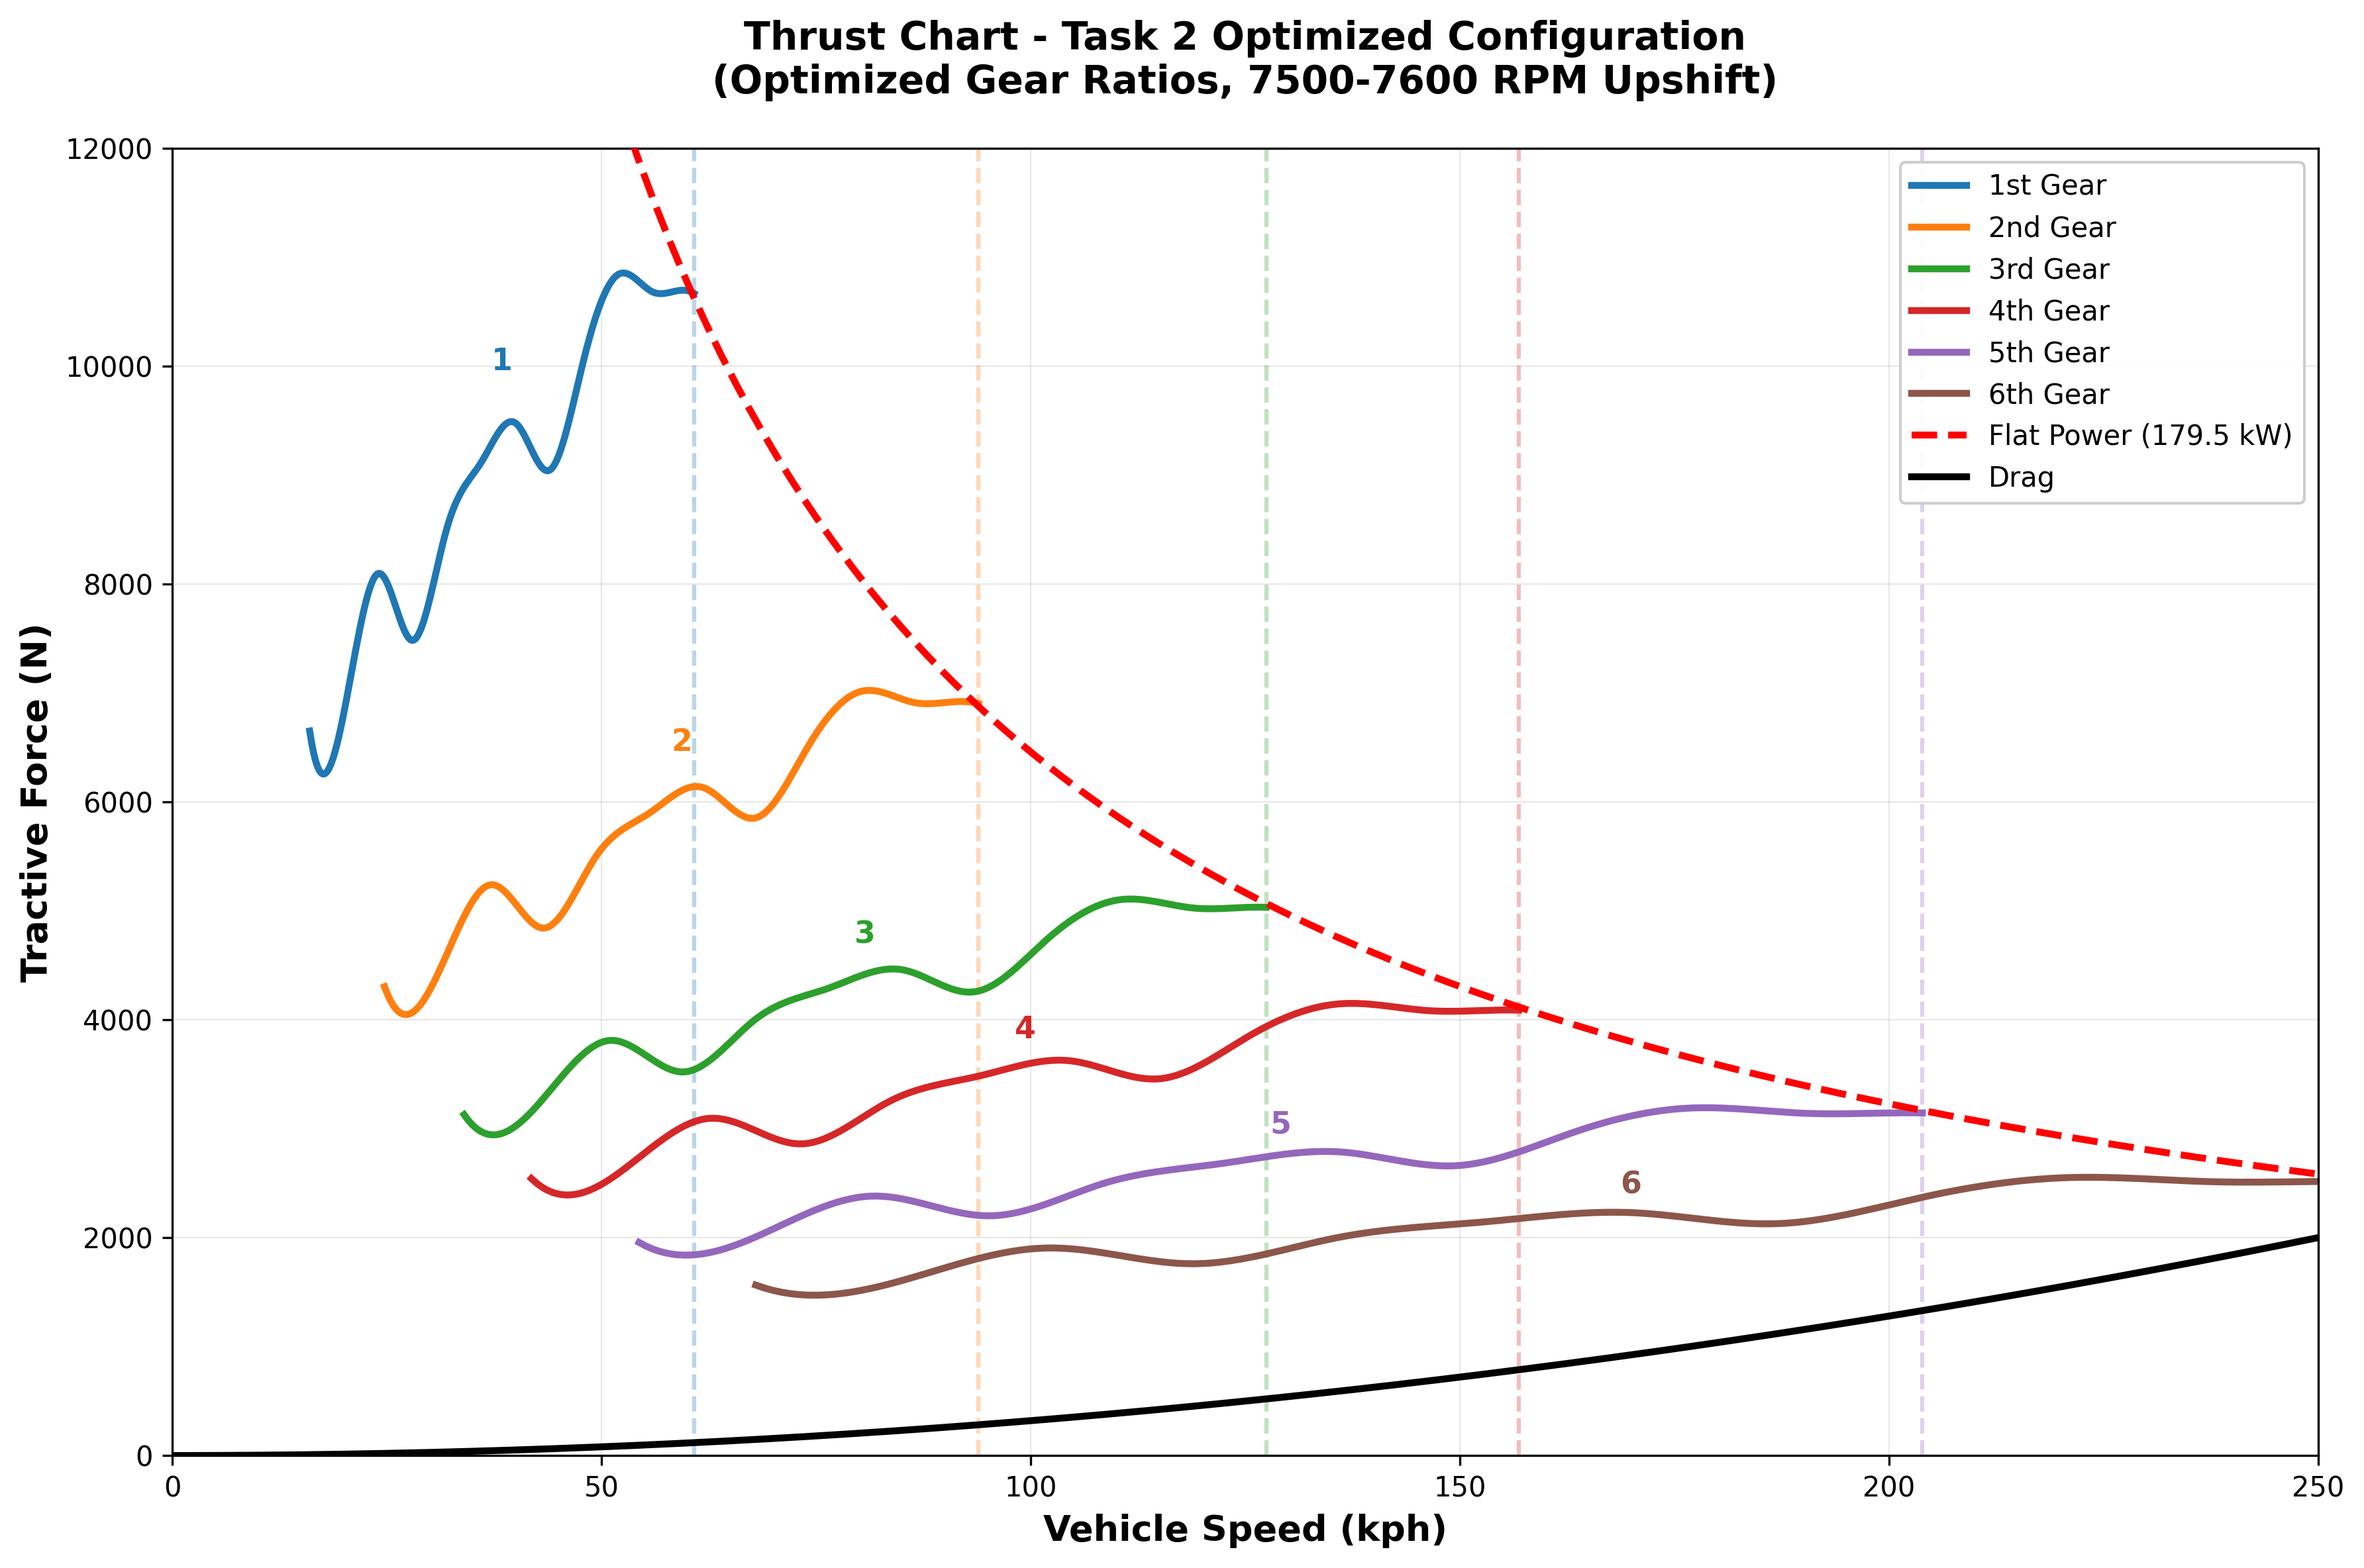
\includegraphics[width=0.75\textwidth]{task4/data/thrustcharts/thrust_chart_optimized_v2.png}
    \caption{Task 2 thrust chart (7500--7600 RPM upshift). The optimized strategy maintains engine in the high-RPM power band (6500--8000 RPM), with gear curves approaching the flat power hyperbola closely throughout the acceleration run. Flat power curve (red dashed) represents theoretical constant power delivery at 179.5 kW.}
    \label{fig:task2_thrust_optimized}
\end{figure}

\begin{figure}[H]
    \centering
    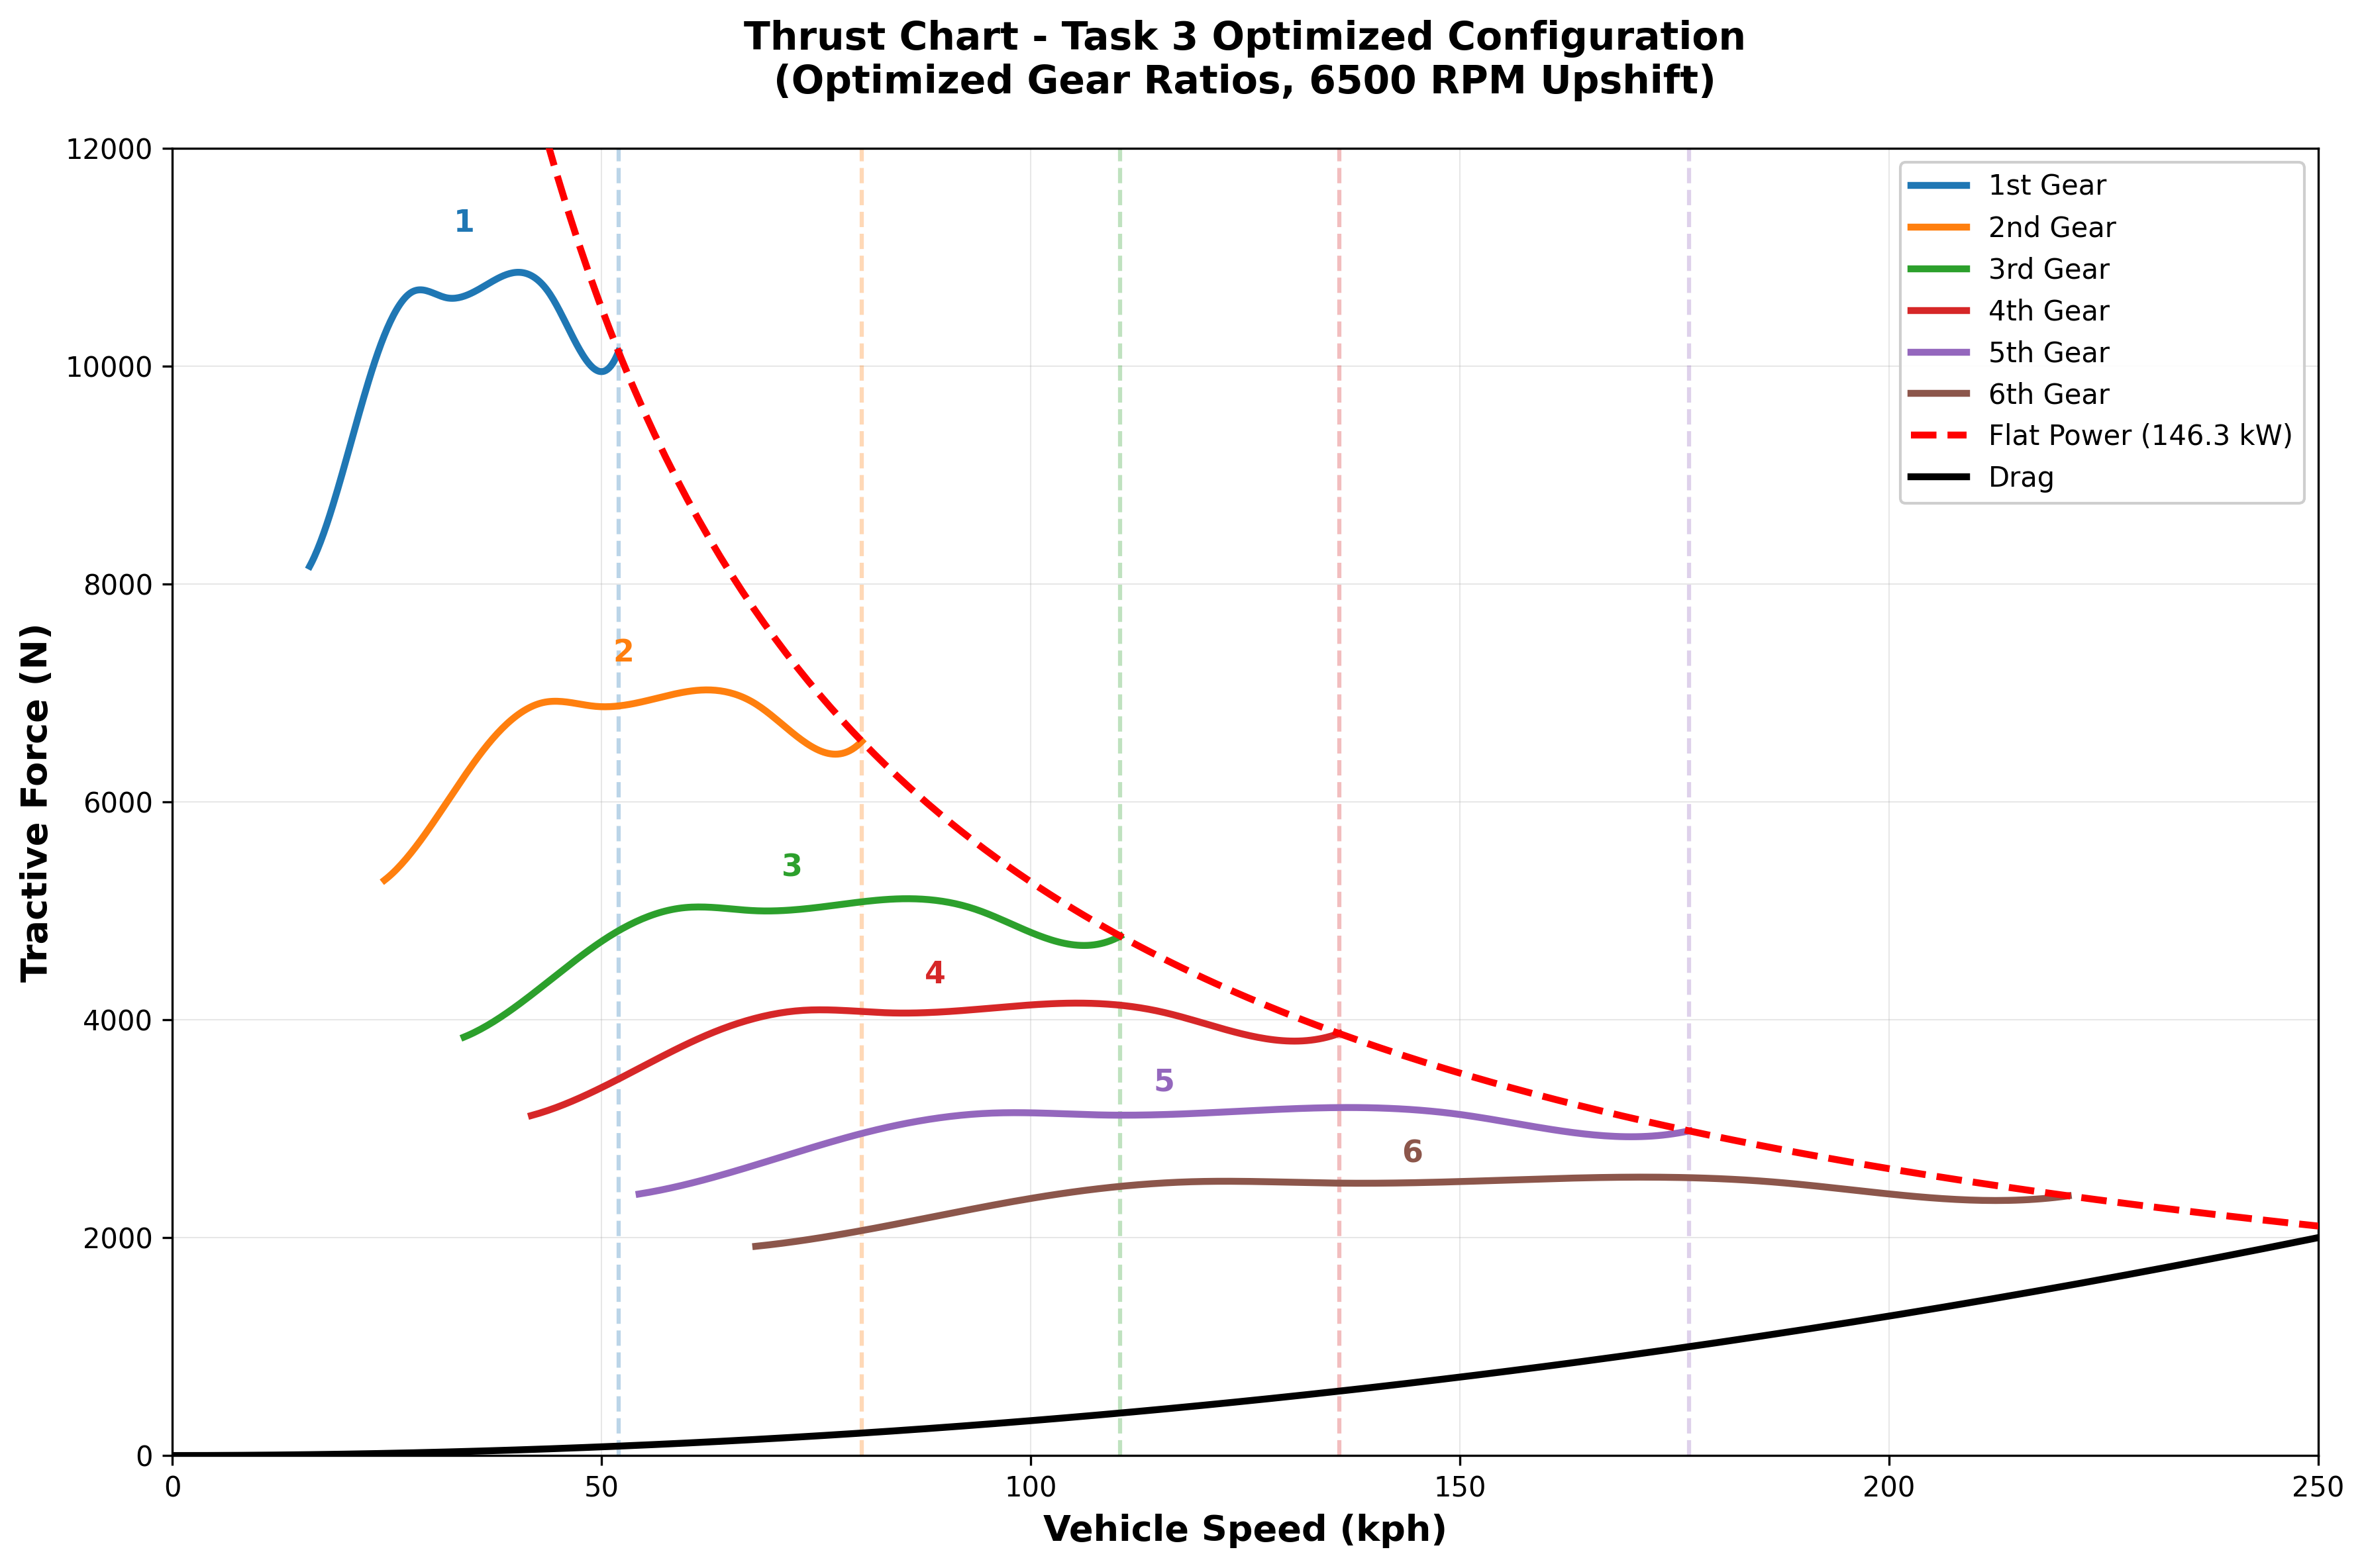
\includegraphics[width=0.75\textwidth]{task4/data/thrustcharts/thrust_chart_task3_optimized.png}
    \caption{Task 3 thrust chart (6500 RPM upshift). The optimized strategy maintains engine in the boost-developed region (3500--6500 RPM). Flatter gear curves compared to Task~2 reflect the turbocharged engine's superior low-to-mid range torque delivery, characteristic of forced induction.}
    \label{fig:task3_thrust_optimized}
\end{figure}

The thrust analysis reveals fundamental differences between the two configurations:

\begin{itemize}
    \item \textbf{Task~2:} Higher peak forces at high speeds due to superior peak power (179.5~kW vs 146.3~kW), but requires high-RPM operation for optimal performance
    \item \textbf{Task~3:} Flatter, more consistent force delivery across speed range due to broad turbo torque plateau (3500--6500~RPM)
    \item \textbf{Top speed:} Task~2 achieves ~208~kph in 6th gear, Task~3 reaches ~221~kph despite lower power, due to taller gear ratios exploiting the full 6500 RPM range
    \item \textbf{Low-speed advantage:} Task~3 delivers higher force at low speeds (below 80~kph), explaining superior 0--100~kph time (4.6s vs 5.2s)
    \item \textbf{High-speed advantage:} Task~2's higher peak power enables faster 0--160~kph time (10.3s vs 11.1s)
\end{itemize}

\subsection{Power Deployment Analysis}

\paragraph{Task~2 Power Sharing:}
The EM contribution is most significant during the 0--40~mph phase, providing up to 30\% of total system power during launch. By 80~mph, the EM contributes approximately 10--15\% of system power.

\paragraph{Task~3 Power Sharing:}
The turbocharged engine benefits from the more powerful Nissan EM61 motor. The EM provides approximately 35--40\% of system power during the 0--40~mph launch phase, significantly more than Task~2 due to the EM61's higher power capability (80~kW vs 25~kW). The EM61's contribution remains substantial at higher speeds (20--25\% of system power), helping to extend the effective power band where the turbocharged engine approaches its 6500~rpm limit.

\subsection{Weight Distribution Effects on Traction}

Weight distribution significantly affects vertical tire loads, and hence the friction limit. In this simulation, a 50/50 static weight distribution is assumed with no driver or passenger, and fuel load included. However, during dynamic launch or acceleration, weight shifts rearward, increasing the vertical load on rear tires and enhancing available traction.

If longitudinal weight transfer is considered, the rear axle may momentarily support 55--60\% of the vehicle weight. This increases $F_z$ at each driven wheel:
\begin{equation}
F_z' = \frac{0.6 \times 720 \times 9.81}{2} = 2116\, \text{N per wheel}
\end{equation}

Thus, the new friction limit becomes:
\begin{equation}
F_{x, \text{max}}' = 0.95 \cdot 2116 \approx 2010\, \text{N per wheel}
\end{equation}
\begin{equation}
T_{\text{wheel,max}}' = 2010 \cdot 0.302 \approx 607\, \text{Nm}
\end{equation}

This implies that during acceleration, the rear tires can tolerate greater wheel torque before slipping. Therefore, gear shift logic and torque maps should ideally account for transient weight transfer to utilize higher traction margins without inducing slip.

\subsection{Tire Property Effects on Simulation Results}

Tire properties play a critical role in determining vehicle performance during transient conditions, especially in acceleration tests such as the 0--100 mph simulation in Task 4. The tire behavior is modeled using the Pacejka "Magic Formula" in AVL CRUISE M, which defines the relationship between slip ratio and longitudinal force, incorporating nonlinear behavior, load sensitivity, and saturation effects.

The most influential tire parameters include:

\begin{itemize}
  \item \textbf{Friction coefficient} $(\mu)$: Determines the peak tractive force that can be generated before slip occurs.
  \item \textbf{Vertical stiffness} $(C_z)$: Affects how load is transferred between tires under acceleration, braking, or cornering.
  \item \textbf{Slip stiffness} $(C_x)$: Governs how quickly force builds up with increasing slip ratio.
  \item \textbf{Rolling radius} $(r)$: Directly influences torque transmission and effective gear ratio.
\end{itemize}

In the current simulation, tire size is set to 195/65R15, resulting in an approximate rolling radius of 0.302 m. With a rear-wheel drive layout and 50/50 static weight distribution, each rear tire supports roughly 1764 N under static conditions. During dynamic acceleration, this load increases due to longitudinal weight transfer, enhancing grip up to a point.

The implications of tire characteristics on simulation outputs are as follows:

\begin{itemize}
  \item \textbf{Acceleration Time:} A higher friction coefficient and optimized vertical load increase the peak tractive force, allowing for faster acceleration. Underestimating $\mu$ leads to premature wheel slip and torque limiting.
  \item \textbf{Wheel Slip Ratio:} Steeper slip curves result in quicker force response but may cause instability under high torque. Proper tuning ensures controlled slip in early gears.
  \item \textbf{Gear Shift Strategy:} If tires cannot transmit high torque at low gears, early upshifting may be required to avoid slipping, compromising acceleration.
  \item \textbf{Torque Limit Tuning:} Wheel torque limits are set based on tire grip; overestimation leads to unrealistic simulation results, while conservative values may underpredict performance.
\end{itemize}

Overall, accurate tire modeling ensures that the simulation reflects realistic vehicle dynamics, traction behavior, and energy efficiency. In Task 4, respecting the tire force envelope is crucial for evaluating whether engine torque and gear strategy can achieve the desired acceleration without exceeding the physical traction limits.

\subsection{Key Findings}

\begin{itemize}
    \item The Task~2 NA engine's high-RPM torque peak required aggressive shifting strategies and substantial EM compensation at low speeds, delivering strong high-speed performance
    \item The Task~3 turbocharged engine's early torque peak provided superior launch characteristics and consistent mid-range acceleration
    \item Identical gear ratios proved effective for both engines despite vastly different torque characteristics
    \item Optimized shifting strategies maintained both engines within optimal operating ranges for 70--90\% of acceleration events
    \item The P1 hybrid architecture effectively integrated with both powerplants using different electric motors: Valeo 48V (25~kW) for Task~2 and Nissan EM61 (80~kW) for Task~3
    \item Different EM power envelopes required tailored calibration strategies for each engine's torque characteristics
    \item Thrust analysis verified that gear ratio optimization successfully maintained engines in optimal RPM ranges while highlighting areas for traction-focused improvement
\end{itemize}

\subsection{Practical Implications}

\begin{itemize}
    \item \textbf{Circuit racing:} NA configuration advantageous through higher peak power
    \item \textbf{Launch performance:} Turbocharged configuration delivers superior low-to-mid speed characteristics
    \item \textbf{Both applications:} P1 hybrid architecture successfully enhances performance regardless of base ICE configuration
\end{itemize}

\subsection{Limitations and Future Work}

\subsubsection{Traction Limit Considerations}

While this study successfully optimized gear ratios for engine operating characteristics and demonstrated effective hybrid integration, several limitations warrant acknowledgment:

\paragraph{Gear Ratio Optimization Scope:}
Due to project time constraints, gear ratio optimization focused primarily on maintaining optimal engine RPM ranges (Task~2: 6500--8000~RPM, Task~3: 3500--6500~RPM) rather than explicit traction envelope matching. The thrust analysis revealed that lower gears generate tractive forces significantly exceeding theoretical tire grip limits:

\begin{itemize}
    \item 1st gear: Approximately 10,500~N peak force versus 4,238~N traction limit ($\mu = 1.2$, FWD, 360~kg front axle), representing 2.5$\times$ excess
    \item 2nd gear: Approximately 6,800~N peak force, still 1.6$\times$ above traction capacity
    \item Addition of P1 electric motor torque further compounds excess force in traction-limited scenarios, particularly during launch
\end{itemize}

\paragraph{Simulation Assumptions:}
The AVL Cruise-M transient simulations assume ideal traction management without explicit wheelspin modeling in the control strategy. Consequently:

\begin{itemize}
    \item Reported 0--100~mph times represent theoretical performance assuming perfect traction control intervention
    \item Actual acceleration times would likely be longer due to traction control limiting, wheelspin events, and driver modulation requirements
    \item Lower gear performance is optimistic, as peak forces exceed available grip by substantial margins
    \item The comparison between Task~2 and Task~3 remains valid as both configurations face similar traction limitations
\end{itemize}

\subsubsection{Recommendations for Future Development}

\paragraph{1. Traction-Optimized Gear Ratios:}
Future iterations should redesign lower gears with traction constraints as primary criteria:
\begin{itemize}
    \item 1st gear: Target ratio 2.5--2.7 (from current 3.4) to limit peak force near traction envelope ($\sim$4,500--5,000~N)
    \item 2nd gear: Target ratio 1.7--1.9 (from current 2.2) to operate closer to available grip
    \item 3rd--6th gears: Maintain current ratios as these operate in power-limited rather than traction-limited regime
\end{itemize}

This approach would improve real-world acceleration performance despite potentially longer simulated times, as traction-optimized ratios enable more effective power delivery to the road surface without excessive wheelspin.

\paragraph{2. Enhanced Traction Modeling:}
Implement dynamic traction management in simulation framework:
\begin{itemize}
    \item Tire slip ratio calculations for realistic wheelspin modeling using Pacejka Magic Formula parameters
    \item Explicit traction control system logic limiting torque to available grip based on real-time slip detection
    \item Variable friction coefficient accounting for vertical load transfer during acceleration
    \item Weight transfer effects on front axle loading for FWD configuration, particularly during high-torque launch phases
\end{itemize}

\paragraph{3. Multi-Objective Optimization Framework:}
Future gear ratio optimization should employ algorithms considering:
\begin{itemize}
    \item Traction envelope constraints as primary design criteria for gears 1--2
    \item Engine RPM optimization as primary objective for gears 3--6 (power-limited regime)
    \item Shift frequency minimization across target speed range to reduce drivetrain losses
    \item Hybrid torque blending strategies maximizing combined ICE+EM output without exceeding grip limits
    \item Launch control strategies for optimal weight transfer utilization
\end{itemize}
